\section{Title: Assessing Discrimination against Women and Underrepresented Minorities in Engineering and the Protective Impacts of Micro-climates}
\section{Introduction}
\label{sec:intro}

 
Engineering is a challenging discipline to study, made more so for students from groups traditionally underrepresented in the field who deal with discrimination, bias, microaggressions, and “othering” during their careers. These groups include racial and ethnic minorities (\eg \cite{Mcgee:2011}), women (\eg \cite{Moss-Racusin:2012}), LGBTQIA+ identifying students (\eg \cite{Cech:2011}) and first-generation college students (\eg \cite{Pascarella:2004,Carrigan, et al., 2019}). Challenges can be compounded when multiple identities come into play (\eg \citep{Williams:2014}). Despite significant funding and attention paid to diversity in engineering, the percentage of B.S. degrees awarded to women engineers in 2017 has increased by just 3\% over 2008 numbers, from 18\% to 21\% \citep{yoder2012engineering}. 
%\sandy{Couldn't this be (mis)interpreted as 'moving in the right direction'?}\jen{better?}

%%\eve{The following paragraph is more about faculty (except for the STEM lab manager work).  do we want more student references?}
 
Although the experiences of minority populations have long been studied, how to increase inclusiveness remains an intractable problem. Discriminatory encounters are ubiquitous, occurring in varied contexts from social interactions with peers, to workplace environments, to stores, to encounters with law enforcement, to educational settings \cite{Fisher:2000}. Experiences of discrimination are undeniably consequential for the life trajectory of young people, particularly students. For example, discrimination, bias, micro-aggressions, and other forms of ``othering'' discourage many minorities from pursuing education in fields that are dominated by the privileged majority (\eg \cite{robinson2015racial}), such as Engineering. Discrimination goes beyond the perceptions of the individual facing to directly impact success in the field. For example, \citet{Moss-Racusin:2012} show that students' resumes with randomly assigned male names are rated as more competent, hireable, and worthy of more mentoring and pay than those same resumes when they are randomly assigned a female name. Research at the University of Washington showed that male students in an undergraduate biology course ranked their male peers as knowing more about the course content than female peers who were performing even better in the class; the authors hypothesize that women's performance is undervalued, they may be more likely to leave a STEM discipline\citep{Grunspan:2016}.
% An earlier psychology study of 238 faculty who received four gender-randomized resumes showed similar outcomes \citep{Steinpreis:1999}. 

It can be particularly difficult to effectively measure the impact of problems, and of solutions, on students. \jen{really need more literature, and justification for why this is tough. How much have students, particularly engineering students, been studies?} %Such research must be  specific and focused. %For example, regarding the question of bias against women, it can be difficult to prove its existence and relationship to gender. 
%%With respect to resume assessments, for example, researchers have measured gender bias by varying only the name (and nothing else) on a resume; using this approach, multiple studies have demonstrated bias. 
%Bias faced by In one recent double-blind study, for example, 127 faculty in Biology and Physics at R1 universities each reviewed an undergraduate resume with a randomly assigned female or male name of an applicant for a fictional lab manager position \citep{Moss-Racusin:2012}. Men were rated as being more competent, hirable, and worthy of mentoring and higher pay than women. Reviewer gender, seniority, field, and age had no effect on outcome.
The impact of such biases hard to measure, since impact may be small and take years to accumulate. %In addition, the studies have mostly focused later in the career such as on The impact of small differences in the evaluation of female candidates of 1-5\% (due to gender bias in performance ratings \citep{Barrett:1993}) can simulate how discrimination will impact gender distributions over time in an organization \citep{Martell:1996} as well as productivity \citep{Cole:1991}. In simulation, these differences lead over time to approximately a 2:1 \paula{I am not sure I understand what the 1-5 and 2:1 references mean here. useful to clarify?} difference in hires of men vs women at the most senior levels \citep{Cole:1991,Martell:1996}. \sandy{This statement also makes little sense to me. What 'measures of success' were studied? Don't they more tellingly affect the number of women who even rise to senior levels?} \jen{need to double check this, but I think it's clearer?}
%More recently, a 2014 study showed that female instructors received lower student evaluations for teaching an online course than males if students believed they were female.  This occurred {\it even if the instructor was actually a male.} This study examined an introductory course in anthropology/sociology, a field with a much higher population of female students than engineering \cite{MacNell:2014}.  
%% Here is the ref: L. MacNell, A. Driscoll, and A. N. Hunt.  What's in %%a name: exposing gender bias in student ratings of teaching. %%{\Innovative Higher Education}, 40(4): 291-303, 2014. 

%After decades of work, researchers have developed a model of impact but still no solution -- no field-tested technique for reducing either bias or its impact.\paula{I like this framing but do not know the discrim intervention literature sufficiently well to know if this statement is supported; there are NO field tests for discrimination reduction? or is the intent to say we don't yet have higher ed based interventions?}%Further, research to date has focused almost entirely on resume assessment of women, a small piece of the much larger picture for minority students attempting to succeed in their fields. How, then, can we expect to solve these problems? \eve{The social psychology literature includes a lot more than resume assessment of women.}

%%\jen{Help... my old segue was flawed... what's the right new one?}

%%\eve{I think the transition reads better by deleting this sentence -- We strongly believe that a far more comprehensive approach to data collection is needed.}

In this era of big data, a comprehensive change in how we collect and assess data about the college student experience is possible. We can now move from lab to field, connect action to behavior, and collect longitudinal data. This, in turn, makes it possible to understand bias in  new ways.  

A 2014 study demonstrates that large-scale, longitudinal data collection can facilitate our understanding of depression and other mental health factors and how they relate to student outcomes (\eg \cite{wang2014studentlife}). That study depended on occasional survey questions combined with a large amount of passive data collection. By complementing self reports with passive data collection, we can similarly use big data to create an image of behavior while learning about specific challenges underrepresented minority engineering students face. This ability to connect behavior to experience in the field was lacking in past studies.  %information about discrimination and bias in the field that can help us understand it better. \sandy{I'm not sure I understand what previous sentence means. Can you clarify what 'connecting behavior to experience' means?}

We now have the technological innovations needed to make this connection possible because we can access devices that passively capture many student activities. %, and there are technical approaches \sandy{such as?} for actively capturing other information we need to know.
Ours is an exciting era for data collection and analysis, one where it is possible to study issues such as discrimination, bias and related adversity exposure at scale and in real-time to understand their various impacts. This important information will help support the design of effective interventions, policies, and decision making to improve the experiences of not just diverse students in engineering, but of all students in engineering. 
 
These insights led us to raise seed money to launch a pilot study with 200 students in 2018. Since then, we have revised our study protocol to further improve it; completed an initial analysis we discuss in this proposal; and begun year one of data collection with a new cohort of 200 first-year students. In both the pilot  and year-one studies, we ensured inclusion of a representative sample of underrepresented groups in engineering (UREs), as shown in Table~\ref{tab:study-participants}. This includes women, underrepresented minorities, first-generation college students, and LGBTQ students. 

While we are still collecting year-one data as of this writing, our pilot data showed high compliance and the significance of the rich, varied data we collected for understanding discrimination. Ninety-one participants from the pilot study reported almost 450 separate instances of discrimination, and we demonstrated the impact of these experiences on their sleep and phone use and connected these behaviors to emotional state.  \paula{below the term challenges is used. This is fine but we will need to think about wording consistency. I used adversity exposure above and we use negative events later. At some points we will be pulling from our fuller data such as MLEs, poverty, ACEs, etc as part of a broader stress assessment within which discrimination is embedded. }
%Our  data show that all of these groups are at risk for discrimination and other obstacles that may impact retention. Further, we argue that an intersectional approach is critical to understanding the challenges these groups face. Thus, we consider discrimination, harassment, and other challenges together with a range of identities in a single holistic study.  

We propose to follow as many of the 200 students from the year-one study as possible for an additional three years to fully understand the longitudinal impact of discrimination on engineering students’ experiences and success. While the data from year one reveal short-term impacts of discrimination, additional data will confirm our observations thus far and shed more needed light on critical long-term impacts, such as retention. \eve{Didn't data from both the pilot and year-one studies show impact of discrimination or do you just mean the pilot here?}

\subsection{Intellectual Merit}
\label{sec:questions}

Our proposed work will leverage the data collected thus far to improve our theoretical understanding of the impact of discrimination on students; answer important questions about both short- and long-term impacts of discrimination; illuminate mediating factors, such as other forms of adversity exposure and resilience as well as influences of micro-climates; and ultimately support intervention design. \paula{I revised above as the figure does not portray micro-climates in a mediating role but seems more related to capturing nuances of key micro-climates.} We  propose to test a model of the student experience (shown in Figure~\ref{fig:model}) that we believe helps capture the differential stressors experienced by women and minorities in engineering in a way that can ultimately be quantified and operationalized. 

\jen{add discussion of rich ema and behavioral data; possibly add interviews; sample size: can we argue for a larger survey? Or for big data within people? methodological solutions? How do we address stability and analysis. rich small data rather than big data}

As shown in Figure~\ref{fig:model} and described in more depth in Section~\ref{sec:back}, much is known about the relationship between the overall stress burden faced by students from different backgrounds, discrimination and long-term stress outcomes, such as physical and mental health \paula{I don't know if more refs are useful but Pascoe & Richman 2009 offer a meta-analysis and similar model that may be worth a look. I have the pdf} (\eg \cite{Ong:2009}). However, many open questions remain, which will constitute the focus of our work; these are shown in Figure~\ref{fig:model} in the boxes with dashed lines along the dashed arrows. We intend to answer four primary questions. \eve{However there are 10 RQs below.} Here, we discuss and explain the importance of each.

\begin{figure}
    \centering
    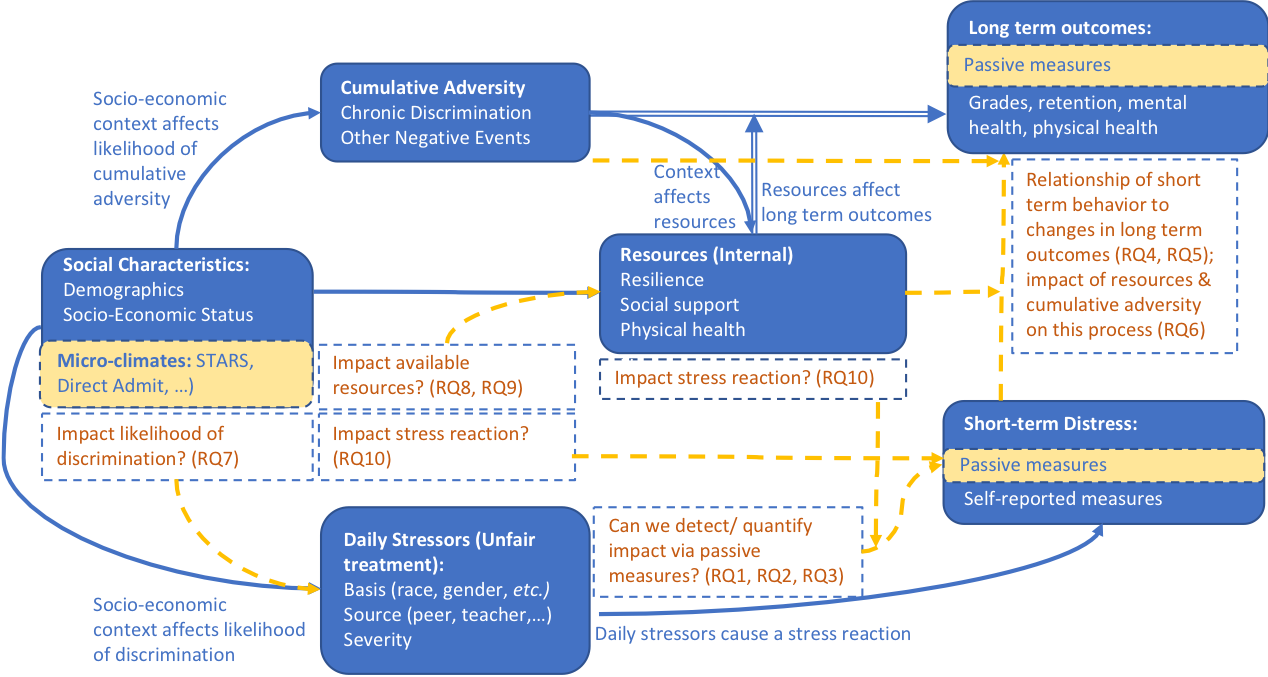
\includegraphics[width=12cm]{img/discrimination-model.png}
    \caption{Theoretical model relating student experiences to long-term outcomes.}
    \label{fig:model}
\end{figure}


\paragraph{Daily Discrimination $\rightarrow$ Short-Term Behavior} Our pilot study already revealed almost 450 separate instances of  \textit{daily discrimination} together with extensive passively-collected behavioral data, unlike any other study. Thus, our first research questions ask what we can learn about the impact of daily discrimination from behavioral data. This is particularly important in an educational context, where we may find, for example, that discrimination is both more likely at high-stress times (such as midterms) and more impactful at these times (if students lose sleep and are thus less well prepared). 
\begin{enumerate}[start=1,label={\bfseries RQ\arabic*}, leftmargin=1cm]
    \item \label{itm:rq-behavior} What is the impact of daily discrimination on short-term behaviors? \paula{the model suggests to me that this question also encompasses effects of the mediating factors. That any given discriminatory event does not carry "pure" effect. Do we want to "set up" in intro analysis re consideration of effects of mediating variables in conjunction with discrimination? If that seems confusing or problematic, cool. if we'd like to consider other analytic approaches, such as \cite{Ong:2009} \textit{et al.'s} attention to negative effects, am happy to discuss. } We hypothesize that this impact is similar to that for stress, which leads to the following question.
    \item \label{itm:rq-behavior-size} Can we quantify both the scope of any behavior change due to a daily discrimination event, and the length of time it is likely to persist? 
    \item \label{itm:rq-severity-impact} Does the severity of the discrimination event(s) change these outcomes?
\end{enumerate}

\paragraph{Short-Term Behavior $\rightarrow$ Long-Term Outcomes} Our second set of questions follows from the first by extending findings to a longitudinal data set. While the impact of discrimination on long-term outcomes has been studied, no prior data set has been able to relate both short- and long-term impacts as we intend to do. \eve{say more about how LT and ST relate}
\begin{enumerate}[start=4,label={\bfseries RQ\arabic*}, leftmargin=1cm]
    \item \label{itm:rq-short-long} Which long-term outcomes are linked to short-term behavior changes, and to what degree? \sandy{Note that many of these questions make assumptions, e.g., that long-term outcomes ARE linked to s-t behavior changes.  Should you ask the question, "Are long-term outcomes linked to short-term behavior changes? How, and to what degree?}
    \item \label{itm:rq-which-long} Are some short-term changes more likely to relate to long-term impacts than others? \paula{We may not want to pursue it, but the model illustrates the capacity to assess daily discrimination and mediating factors as co-contributors to long term impacts. I am finding myself unclear how to think about short term behaviors as major contributors aside from stressors as key contributors to long term behavior and well being}
    \item \label{itm:rq-severity-long} Do specific factors, such as cumulative impact of discrimination or number of repetitions, predict long-term impacts? \paula[again, do we want to frame this as looking at cumulative discrim in conjuction with chronic discrim and other adversities or negative events?]
\end{enumerate}
 
\begin{WrapText}
\begin{description}[leftmargin=1cm]
\item[STARS] The Washington {ST}ate Academic RedShirt (STARS) program supports engineering and computer science students from low-income, first-generation, and underserved backgrounds in navigating the transition to college.
STARS is a two-year program with a specialized curriculum designed to build learning skills and strengthen academic preparation for core math and science prerequisites. STARS scholars are guaranteed placement into an engineering or computer science major.

\item[Introductory Sequence] The introductory course experience can significantly affect the likelihood of discrimination due to the level of competitiveness...
\item[SEEEDS Bridge Program] Through the Summer Early Enrichment in Engineering for Dean's Scholars (SEEEDS), incoming first-year engineering students, who come from underserved backgrounds but do not necessarily need or want the intensive STARS intervention, get support to succeed in their first prerequisite courses at UW.  They also build community and learn about the myriad academic and professional development resources for UW students. 
\item[FIGS?]
\end{description}
\end{WrapText}

 \paragraph{Micro-Climates $\rightarrow$ Indirect Impact} Although novel intervention design is beyond the scope of this proposal, we intend for the proposed work to clarify the impact of existing micro-climates, which can in turn guide intervention design. We have already identified multiple micro-climates that could affect the discrimination-stress process highlighted in Figure~\ref{fig:model}, including the Washington \textbf{St}ate \textbf{A}cademic \textbf{R}ed\textbf{S}hirt (STARS) program; introductory course sequences that students must take; and participation in the Summer Early Enrichment for Engineering for Dean's Scholars (SEEEDS) bridge program (see Sidebar~\ref{sidebar:definitions}). \paula{useful to define earlier or here what micro-climates are defined as? \Sandy {Yes, please define this term.} how will negative micro-climates or those beyond the noted groups be assessed? do settings like labs or other routine places respondents spend time considered micro-climates?} We believe that these micro-climates will indirectly affect outcomes through their impact on mediating factors and the likelihood of daily discrimination events. \eve{what are mediating factors? What do we mean by their impact}\jen{we probably need to decide whether to say mediating or moderating. Could be a question for Paula}
 
\begin{enumerate}[start=7,label={\bfseries RQ\arabic*}, leftmargin=1cm]
    \item \label{itm:mc-daily-discrimination} Which micro-climates will reduce exposure to daily discrimination? Which micro-climates will increase exposure?\sandy{Again, rephrase:  Will micro-climates reduce/increase exposure to daily discrimination?}

    \item \label{itm:mc-external-mediators} Which micro-climates will increase or decrease external mediating factors, such as exposure to negative events? Will this translate into different short- or long-term behavioral outcomes using the mechanisms identified in the prior RQs?
    \item \label{itm:mc-internal-mediators} Which micro-climates will increase or decrease internal mediating factors, such as resilience and two-way social support? Will this translate into different short- or long-term behavior outcomes using the mechanisms identified in the prior RQs?
    \item \label{itm:mc-mediators-behavior} How important are mediating factors to short term behaviors (to what extent to they cause responses to be much larger or smaller?). How does this impact the translation of short term behavior into long term outcomes?
\end{enumerate}
 
We seek to develop a holistic understanding of the impacts of discrimination on the participation and retention of UREs throughout  their college career. Specific contributions of our work will include: (1) a \textbf{more complete theoretical model} of the impact of discrimination than those provided in previous work.  Our research will also make it possible: (2) to document, for the first time, \textbf{what behaviors change and in what ways} following acts of discrimination, and (3) to demonstrate, for the first time, \textbf{which micro-climates reduce that impact and through what mechanisms}. Finally, this in turn can (4) guide the \textbf{development of interventions }that help to mediate or reduce the experience of discrimination.  

\subsection{Broader Impacts}
\noindent
Our proposed work will improve outcomes for UREs by: (1) \textbf{quantifying impact of unfair treatment} (i.e., discrimination, harassment, etc.)  on students; (2) \textbf{demonstrating to what degree discrimination impacts the success and retention} of underserved groups; and (3) \textbf{quantifying the protective impact of a currently deployed intervention (STARS)}, an intentionally created micro-climate targeting the most under-prepared  students in Engineering and Computer Science. 

The University of Washington is one of 8 or 10 large flagship public universities in the country. \Sandy{hmmm, it's not in top 10 in terms of enrollment - https://www.stilt.com/blog/2018/01/americas-10-largest-universities-enrollment/.  What does "flagship" mean here?} Student experiences in different university settings are likely to be similar in terms of program scale and the range of students and student backgrounds entering the engineering program. This makes it likely that similar interventions will work in similar ways. The impact of discrimination on mental and physical health is already well-demonstrated in multiple studies. Thus, we expect that our findings will translate to similar large public universities, meaning that we have the potential to impact X 1000 engineers in training each year. We believe that our work will translate to engineering programs at other universities that are working to increase their diversity, as well. 

To this end, we will disseminate the results of our proposed research to other universities working to retain underserved students in Engineering and Computer Science.  Co-PI Riskin is PI of the UW STARS program, which was founded at UW and Washington State University in 2013 and is now entering its 7th year at both universities;  STARS is an adaptation of the Goldshirt Program at the University of Colorado, Boulder, now entering its 11th year. Through UW’s leadership, the `redshirt' model has since been adopted at three additional institutions through a six-institution Redshirt in Engineering Consortium grant from the National Science Foundation (UW, WSU, University of Colorado, Boulder, University of Illinois, Urbana-Champaign, Boise State University, and University of California, San Diego). Through the Redshirt Consortium, UW is engaged in sharing best practices to support first-generation students and students from low-income backgrounds. 

In the remainder of this proposal, we describe the pilot study that we have already conducted. We also present a simple, preliminary analysis of our data, which demonstrates the promise that our approach can indeed support investigation of our important research questions R1-R10.
 
\subsection{Team}
 
Jennifer Mankoff is the Richard E. Ladner professor in the Paul G. Allen School of Computer Science and Engineering. She has worked with underrepresented populations for over a decade (\eg \cite{newman2004perceptions,DBLP:conf/huc/DillahuntMPF09,DBLP:conf/cscw/DillahuntM14,DBLP:conf/huc/DillahuntMP10,DBLP:journals/pacmhci/EarlyHHRWM18,DBLP:conf/chi/OLearyZMR19}). In addition, she has led the UW EXP effort, helped to build the research team, and will continue to lead the effort over the remaining years of the study. Her background in Human Computer Interaction has prepared her well to conduct research of this scope, and her research includes a mix of qualitative behavioral work (\eg \cite{DBLP:conf/huc/DillahuntMPF09,DBLP:conf/chi/MankoffKKRW11}), mixed-methods/quantitative behavioral work (\eg \cite{DBLP:conf/ph/CrawfordGSAM14,DBLP:journals/pacmhci/EarlyHHRWM18}) and technical work in behavior modeling (\eg \cite{DBLP:conf/chi/BanovicBCMD16}). 
 
Eve Riskin is Professor of Electrical and Computer Engineering, Associate Dean of Diversity \& Access in the UW College of Engineering, founder of the UW STARS program, and Faculty Director of UW's ADVANCE program. She has been working to promote diversity and inclusion in engineering for nearly two decades and has published research both at the student (\cite{carriganactive,myers2018redshirt}) and faculty levels (\cite{carrigan2017ramping,carrigan2011gendered,yen2019promoting}).
 
Paula Nurius is the Grace Beals Ferguson Professor and Associate Dean at the UW School of Social Work. She brings many years of research and training experience in the areas of stress processes and short-term and life-course effects of discrimination, cumulative adversity and social disadvantage among both general and at-risk populations, including students. Prominent outcomes address mental and physical health, school experiences, and prevention and intervention implications (IF CITES NEEDED I CAN PROVIDE SOME). Her background in relevant social science theories, measures, and analytic strategies complements the expertise of other team members. 
